\documentclass[12pt]{article}
\usepackage[brazil]{babel}
\usepackage[utf8]{inputenc}
\usepackage{graphicx}
\usepackage{amsmath}
\usepackage{float}
\usepackage{listings}
\usepackage{algorithmic}
\usepackage{hyperref}


\title{Resumo - Regras de associação}
\author{
Herberth Amaral \\
Departamento de Ciência da Computação\\
Programa de Pós Graduação em Modelagem Computacional e Sistemas\\
Universidade Estadual de Montes Claros - UNIMONTES\\
}
\date{\today}

\begin{document}
\maketitle

\begin{abstract}
    Este documento é um resumo do capítulo 7 do livro Introdução à Mineração de dados (ref?)
\end{abstract}

\section{Introdução}

Uma regra de associação é uma relação "interessante" entre variáveis de
transações em bancos de dados. Entende-se \textbf{transação} como uma entrada
em um banco de dados transacional (ex: PDV -- ponto de vendas -- de um
supermercado) discreto que possui itens binários (ou seja, $\in \{0,1\}$) que
descrevem essa transação (ex: itens da cesta de compras).  Segundo
\cite{agrawal}, o problema é definido como $I = \{i_1, i_2, \ldots, i_n\}$
sendo um conjunto binário de $n$ atributos chamados de itens e $T = \{t_1, t_2, \ldots, t_i\}$ 
como sendo o conjunto de transações chamado de banco de dados. 

Uma regra é definida como $X \rightarrow Y; X,Y \subseteq I; X \cap Y = \emptyset$, 
que basicamente diz que se X ocorreu, então Y também ocorreu. Em
termos de um PDV, se X foi comprado, então Y também foi comprado. Neste caso, X
e Y são atributos transacionais diferentes numa base de dados. Uma regra é
considerada \textit{forte} se há alta coocorrência entre os itens.

Como exemplo prático, uma regra de associação determina a probabilidade da
compra de um ou mais itens em um supermercado levarem a compra de um outro
item. Um caso (provavelmente um mito) conhecido é a relação entre compras de
fraldas e cervejas numa Quinta-feira.

A \textit{mineração de regras de associação} é uma técnica usada na descoberta
de relações sob forma de regras entre itens de uma base de dados transacional.

As regras de associação possuem dois requisitos básicos: \textbf{suporte} e
\textbf{confiança}. Em outros contextos, esses mesmos conceitos são conhecidos
como \textbf{revocação} e \textbf{precisão}. Interessantemente as regras de
associação não trabalham com algo análogo ao escore F1 ($F1 = 2 * \frac{SC}{S+C}$, 
em que S é o suporte e C é a confiança). O suporte a confiança são definidos como:

\begin{center}
    $Sup(A \rightarrow C) = P(A \cup C) = \dfrac{\sigma(A \cup C)}{n}$ \\[2.8ex]
    $Conf(A \rightarrow C) = P(C|A) = \dfrac{\sigma(A \cup C)}{\sigma(A)}$ \\[2.8ex]
    $\sigma(A) = |\{t_i| A \subseteq t_i, t_i \in T\}|$ \\
\end{center}

Existem outras métricas que relacionam o suporte com a confiança. Tais métricas
incluem, mas aparentemente não limitam-se a, Lift, Convicção,
compreensibilidade e grau de interesse. São definidas assim:

\begin{center}
    $Lift (A \rightarrow C) = \dfrac{Conf(A \rightarrow C)}{\sigma(C)} = \dfrac{\sigma(A \cup C)}{\sigma(A).\sigma(C)}$ \\[2.8ex]
    $Conv (A \rightarrow C) = \dfrac{1 - Sup(C)}{1-Conf(A \rightarrow C)}$ \\[2.8ex]
    $Comp (A \rightarrow C) = \dfrac{log(1+|C|)}{log(1+|A \cup C|)}$ \\[2.8ex]
    $Int (A \rightarrow C) = \dfrac{Sup(A \rightarrow C)}{Sup(A)}.\dfrac{Sup(A \rightarrow C)}{Sup(C)}.(1 - \dfrac{Sup(A \rightarrow C)}{n})$
\end{center}

Algumas considerações sobre as métricas:

\begin{enumerate}
    \item O lift parece ser algo mais próximo do escore F1, comumente encontrado na literatura para avaliação de mecanismos de busca. O problema é que o lift nunca chega a 1;
    \item A convicção tende ao infinito à medida que a confiança tende a 1 e a 0 quando o suporte tende a 1.
    \item O grau de compreensibilidade cresce à medida que um menor número de itens é usado na composição das regras de associação. Quanto menos itens, mais fácil de se compreender a regra;
    \item O autor diz que o grau de interesse em uma regra aumenta se ocorrer poucas vezes na base de dados. Aparentemente, quanto mais próximo de 0, mais interessante é.
\end{enumerate}

\section{Algoritmos de mineração de regras}

Como a mineração de regras por força bruta é um processo de complexidade
exponencial, se faz necessário utilizar técnicas mais "inteligentes" para
mineração de regras de associação. Esta seção trata dos principais algoritmos.

\subsection{Algoritmo Apriori}

O algoritmo visa diminuir o custo computacional na mineração de regras através
do desacoplamento dos requisitos de suporte e confiança mínima das regras. Sua
estratégia consiste em:

\begin{enumerate}
    \item Geração do conjunto de itens frequentes;
    \item Geração das regras.
\end{enumerate}

Para diminuir o espaço de busca do algoritmo, pode-se eliminar regras que não
atendam a um suporte mínimo. A eliminação dessas regras começa com a eliminação
de itens não-frequentes. 

A figura \ref{fig:apriori} ilustra o algoritmo Apriori.

\begin{figure}[H]
    \centering
    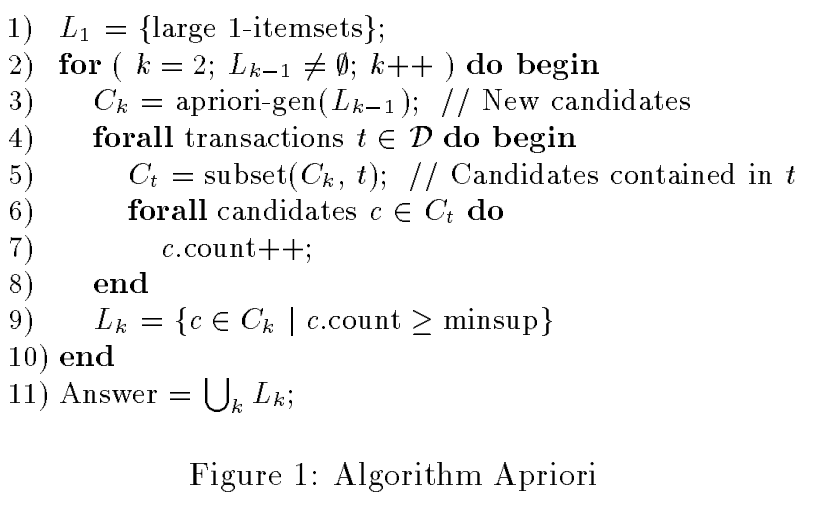
\includegraphics[width=0.8\textwidth]{apriori.png}
    \caption{Algoritmo Apriori \cite{agrawal}}
    \label{fig:apriori}
\end{figure}

A linha 9 mostra a eliminação dos itens não frequentes do conjunto de soluções
que o algoritmo pode fornecer.

O algoritmo Apriori foi um marco importante na mineração de regras, mas ainda
sim é ineficiente para grandes bases de dados com transações contendo muitos
itens.

\subsection{Algoritmo FP-Growth}

O algoritmo FP-growth usa uma abordagem mais interessante que o Apriori: ele
constrói uma lista decrescente de itens mais frequentes e depois constrói uma
árvore de relações que a frequencia vai diminuindo com o aumento da
profundidade.

A determinação dos itens frequentes pode ser feita utilizando uma simples SQL
caso a base de dados em questão seja relacional:

\lstinputlisting[language=SQL]{fpgrowth.sql} 

A FT-tree é criada com os seguintes passos:

\begin{enumerate}
    \item $L \leftarrow itens\_ordenados\_por\_frequencia$
    \item $FT-tree \leftarrow null$
    \item Para cada transação $t \in T$
        \begin{enumerate}
            \item $l \leftarrow itens\_ordenados\_por\_L$
            \item InsertTree(l, FT-Tree)
        \end{enumerate}
\end{enumerate}

A função InesertTree funciona da seguinte forma: se a árvore possui um
descendente D, tal que $D.nome\_do\_item = p.nome\_do\_item$ então incremente a
contagem de D em 1; Senão crie um nó D e atribua 1 à sua contagem, seu nó pai é
ligado à Tree e ele é ligado a todos os nós com o mesmo $nome\_do\_item$. 

\subsubsection{Exemplo}

Este exemplo foi retirado de \url{https://en.wikibooks.org/wiki/Data\_Mining\_Algorithms\_In\_R/Frequent\_Pattern\_Mining/The\_FP-Growth\_Algorithm}.

Considere as transações da tabela \ref{tbl:exemplo}.

\begin{table}[H]
\centering
\caption{Transações de exemplo}
\label{tbl:exemplo}
\begin{tabular}{ll}
TID & Itens \\
1   & ABDE  \\
2   & BCE   \\
3   & ABDE  \\
4   & ABCE  \\
5   & ABCDE \\
6   & BCD  
\end{tabular}
\end{table}

A lista L com os itens ordenados de forma decrescente neste caso é $\{B(6),E(5),A(4),C(4),D(4)\}$

As imagens a seguir mostram a árvore depois da adição de cada transação.

\begin{figure}[H]
    \centering
    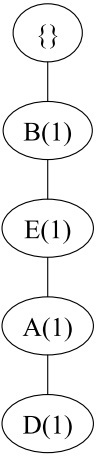
\includegraphics[width=0.1\textwidth]{t1.jpg}
    \caption{FT-Tree depois da inserção da primeira transação}
    \label{fig:apriori}
\end{figure}


\begin{figure}[H]
    \centering
    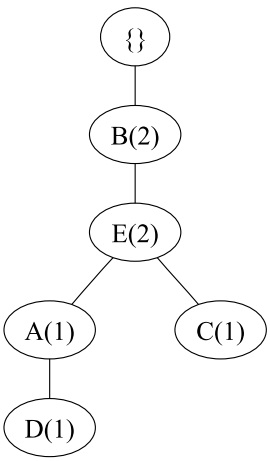
\includegraphics[width=0.2\textwidth]{t2.jpg}
    \caption{FT-Tree depois da inserção da segunda transação}
    \label{fig:apriori}
\end{figure}

\begin{figure}[H]
    \centering
    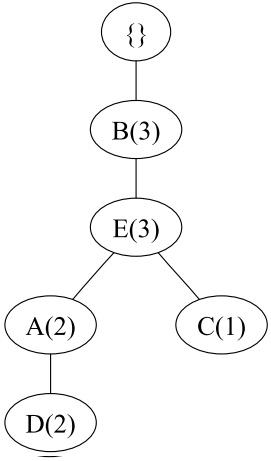
\includegraphics[width=0.2\textwidth]{t3.jpg}
    \caption{FT-Tree depois da inserção da terceira transação}
    \label{fig:apriori}
\end{figure}

\begin{figure}[H]
    \centering
    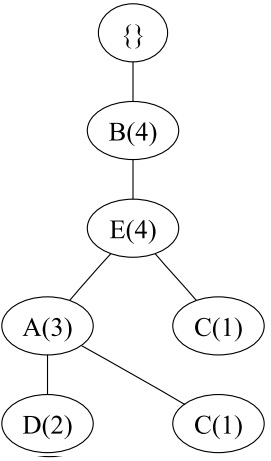
\includegraphics[width=0.2\textwidth]{t4.jpg}
    \caption{FT-Tree depois da inserção da quarta transação}
    \label{fig:apriori}
\end{figure}

\begin{figure}[H]
    \centering
    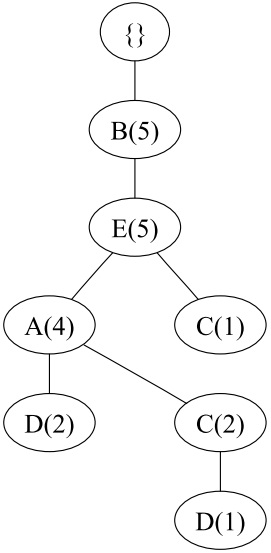
\includegraphics[width=0.2\textwidth]{t5.jpg}
    \caption{FT-Tree depois da inserção da quinta transação}
    \label{fig:apriori}
\end{figure}

\begin{figure}[H]
    \centering
    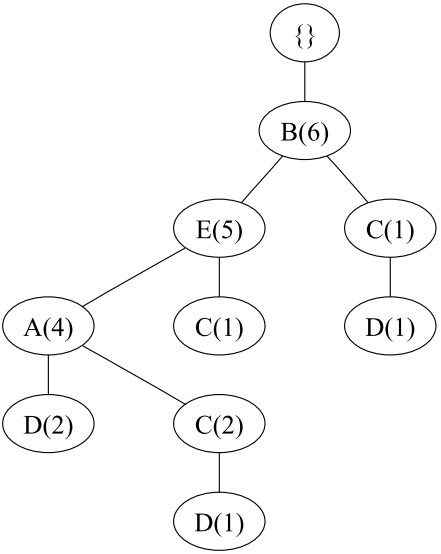
\includegraphics[width=0.2\textwidth]{t6.jpg}
    \caption{FT-Tree depois da inserção da sexta transação}
    \label{fig:apriori}
\end{figure}

É possível observar algumas coisas da FT-Tree:

\begin{enumerate}
    \item É possível que haja mais de uma raiz de árvore. De fato, a árvore vai ter somente uma raiz se \textbf{todas} as transações tiverem um item em comum, o que é bem difícil na vida real;
    \item O FP-Growth é tido como um processo escalável, capaz de ser paralelizado. É possível fazer um \textit{map-reduce} em que o map recebe um conjunto de transações e monta as árvores correspondentes e o reduce faz o "merge" dessas árvores. No entanto, talvez seja mais interessante ter uma estrutura de dados em árvore distribuída para este fim;
    \item O FP-growth tem uma complexidade de espaço na prática bem menor que a complexidade de espaço do Apriori. Em bases de dados relacionais, a geração da matriz binária pode ser um processo caro em uma base de dados SQL, o que diminui ainda mais a eficiência do Apriori;
    \item O FP-growth permite uma visualização mais clara das regras de associação (opinião do autor).
\end{enumerate}

\bibliographystyle{alpha}
\bibliography{resumo}

\end{document}
